% !TEX root = ../TensorOT.tex




%%%%%%%%%%%%%%%%%%%%%%%%%%%%%%%%%%%%%%%%%%%%%%%%%%%%%%%%%
\subsection{Diffusion Tensor Imaging}

Diffusion tensor magnetic resonance imaging (DTI) is a popular technique to image the white matter of the brain (see~\cite{wandell2016clarifying} for a recent overview). DTI measures the diffusion of water molecules, which can be compactly encoded using a PSD tensor field $\mu(x) \in \Ss_+^3$, whose anisotropy and size matches the local diffusivity. 
%
A typical goal of this imaging technique is to map the brain anatomical connectivity, and in particular track the  white matter fibers. This requires a careful handling of the tensor's energy (its trace) and anisotropy, so that using Q-OT is a perfect fit for such data.

Figure~\ref{fig:dti} shows an application of Q-OT for the interpolation (using~\ref{eq-interpolating}) between 2-D slices from DTI tensor fields $(\mu,\nu)$ acquired on two different subjects. This data is extracted from the studies~\cite{pestilli2014evaluation,takemura2016ensemble}. These two patients exhibit different anatomical connectivity geometries, and Q-OT is able to track the variation in both orientation and magnitude of the diffusion tensors. This figure also compares the different data fidelity parameters $\rho \in \{0.05,1\}$. Selecting $\rho=1$ enforces an overly-strong conservation constraint and leads to interpolation artifacts (in particular some structure are split during the interpolation). In contrast, selecting $\rho=0.05$ introduces enough mass creation/destruction during the interpolation to be able to cope with strong inter-subject variability.

%%% FIG %%%
\newcommand{\DTIimg}[1]{\includegraphics[width=.195\linewidth,trim=85 20 85 20,clip]{dti/#1}}
\begin{figure}\centering
\begin{tabular}{@{}c@{\hspace{1mm}}c@{\hspace{1mm}}c@{\hspace{1mm}}c@{\hspace{1mm}}c@{}}
\DTIimg{one-two/interpol-rho1-1}&
\DTIimg{one-two/interpol-rho1-3}&
\DTIimg{one-two/interpol-rho1-5}&
\DTIimg{one-two/interpol-rho1-7}&
\DTIimg{one-two/interpol-rho1-9}\\
\DTIimg{one-two/interpol-rho005-1}&
\DTIimg{one-two/interpol-rho005-3}&
\DTIimg{one-two/interpol-rho005-5}&
\DTIimg{one-two/interpol-rho005-7}&
\DTIimg{one-two/interpol-rho005-9}\\
\DTIimg{four-two/interpol-rho005-1}&
\DTIimg{four-two/interpol-rho005-3}&
\DTIimg{four-two/interpol-rho005-5}&
\DTIimg{four-two/interpol-rho005-7}&
\DTIimg{four-two/interpol-rho005-9}\\
$t=0$ & $t=1/4$ & $t=1/2$ & $t=3/4$ & $t=1$
\end{tabular}
\begin{tabular}{@{}c@{\hspace{2mm}}c@{\hspace{2mm}}c@{}}
\includegraphics[width=.3\linewidth]{dti/one-two/original-trace-1-roi}&
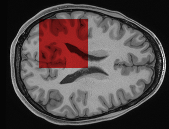
\includegraphics[width=.3\linewidth]{dti/one-two/original-trace-2-roi}&
\includegraphics[width=.3\linewidth]{dti/four-two/original-trace-1-roi}\\
Subject $A$ & Subject $B$ & Subject $C$  
\end{tabular}
\caption{Interpolation between two 2-D slices of 3-D DTI tensor fields $(\mu,\nu)=(\mu_{t=0},\mu_{t=1})$. For readability, only the X/Y components of the tensors are displayed. 
\textbf{First row:} interpolation between subjects $(A,B)$ obtained using $\rho=1$. 
\textbf{Second row:} interpolation between subjects $(A,B)$ obtained using $\rho=0.05$. 
\textbf{Third row:} interpolation between subjects $(C,B)$ obtained using $\rho=0.05$. 
\textbf{Fourth row:} anatomical MRI images of subjects $(A,B,C)$ indicating the region of interest where the computations are performed. 
} \label{fig:dti}
\end{figure}
%%% FIG %%%